
\begin{frame}[plain,c]
\begin{center}
{\Huge \bf Optional reading for Lecture \thislecture}
\end{center}
\end{frame}

% ------------------------------------------------------------------------------

%
% Worked example :
%

{
\problemslide

%
%
%

\begin{frame}{Worked example: Wire loop falling in magnetic field}

  \begin{blockexmplque}{Question}
    A rectangular loop of wire with dimensions $\ell$ and $w$ is released at
    $t=0$ from rest, just above a region in which the magnetic field is
    $\vec{B}_0$, as shown in the figure below.
    $\vec{B}_0$ is perpendicular to the loop of wire.
    \begin{center}
         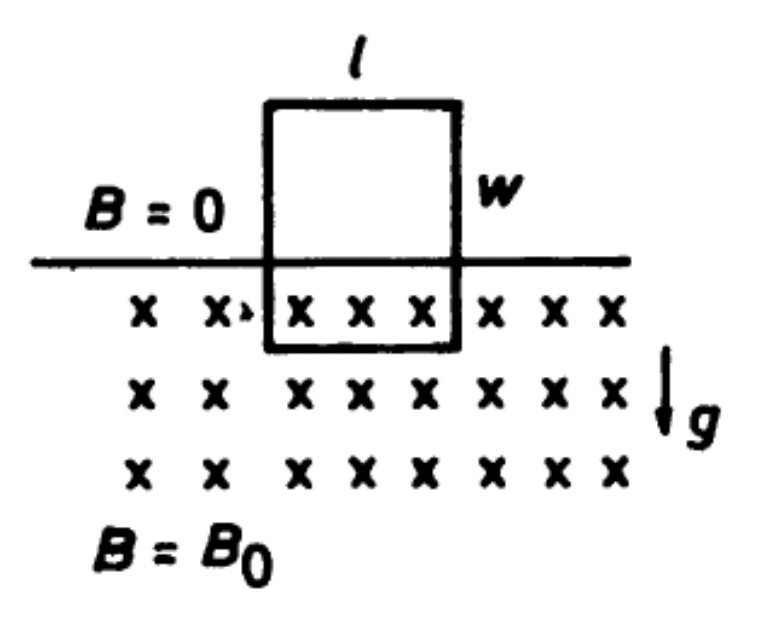
\includegraphics[width=0.35\textwidth]{./images/problems/lect11_wire_loop_falling_in_b_field}
     \end{center}
    The loop has resistance $R$, self-inductance $L$, and mass $m$.
    Consider the loop during the time that it has its upper edge
    in the zero-field region.\\
  \end{blockexmplque}

\end{frame}

%
%
%

\begin{frame}{Worked example: Wire loop falling in magnetic field}

  \begin{blockexmplque}{Question (cont'd)}
    \begin{itemize}
      \item
      Discuss the forces acting on the loop and write
      Newton’s equation of motion for the loop.
      \item
      Find expressions for the electromotive force induced by the motion
      of the loop in the magnetic field, as well as for the voltage drops
      due to the resistance and self-inductance of the loop and relate
      them via Kirchhoff’s voltage law.
      \item
      Assuming that you can ignore the self-inductance of the loop
      but not the resistance,
      find the current and velocity of the loop as functions of time.
      \item
      Assuming that you can ignore the resistance of the loop
      but not the self-inductance,
      find the current and velocity of the loop as functions of time.
    \end{itemize}
  \end{blockexmplque}

\end{frame}

%
%
%

\begin{frame}{Worked example: Wire loop falling in magnetic field}

  %
  % %%% 1
  %

  The loop has mass $m$ and the gravitational force that
  will be exerted upon would be:
  \begin{equation*}
    F_{g} = mg
  \end{equation*}

  At $t$=0, the horizontal (bottom) segment of the loop
  enters the magnetic field. At $t>0$, the magnetic force exerted
  upon that segment is given by:
  \begin{equation*}
    |\vec{F}_{B}| = | I \int_{\ell} d\vec{\ell} \times B | = B_0 \ell I
  \end{equation*}

  The magnetic force will point upwards and will oppose the
  gravitational force with points downwards.\\
  \vspace{0.2cm}

  Newton's law of motion for the loop is:
  \begin{equation*}
    mg - B_0 \ell I = m \frac{du}{dt}
  \end{equation*}

\end{frame}

%
%
%

\begin{frame}{Worked example: Wire loop falling in magnetic field}

  %
  % %%% 1
  %

  The electromotive force (EMF) that will be developed along the
  horizontal (bottom) segment of the loop is:
  \begin{equation*}
    \varepsilon =
      |\int_{\ell} (\vec{u} \times \vec{B}) \cdot d\vec{\ell}| = B_0 \ell u
  \end{equation*}

  The back-EMF due to the inductance L of the loop is:
  \begin{equation*}
    \varepsilon_{back} = V_{L} = - L \frac{dI}{dt}
  \end{equation*}

  The voltage drop due to the resistance R of the loop is:
  \begin{equation*}
    V_{R} = RI
  \end{equation*}

  Kirchoff's voltage law relates the directed sum of EMFs
  with the sum of voltage drops along the loop
  \begin{equation*}
    \varepsilon + \varepsilon_{back} = V_{R} \Rightarrow
    B_0 \ell u - L \frac{dI}{dt} = RI
  \end{equation*}

\end{frame}

%
%
%

\begin{frame}{Worked example: Wire loop falling in magnetic field}

  %
  % %%% 3
  %
  Assuming that $L=0$, Kirchoff's voltage law
  relates $I$ and $u$ as follows:
  \begin{equation*}
    B_0 \ell u - \cancelto{0}{L} \;\; \frac{dI}{dt} = RI \Rightarrow
    B_0 \ell u = RI \Rightarrow I = \frac{B_0 \ell}{R} u
  \end{equation*}

  Substituting the above expression for $I$
  in Newton's law yields:
  \begin{equation*}
    mg - B_0 \ell \Big( \frac{B_0 \ell}{R} u \Big) = m \frac{du}{dt} \Rightarrow
    \frac{du}{dt} = g - \frac{B_0^2 \ell^2}{mR} u \Rightarrow
  \end{equation*}
  \begin{equation*}
    \frac{d(u/g)}{dt} = 1 - \frac{B_0^2 \ell^2}{mR} (u/g)
  \end{equation*}

  By making the following substitutions:
  \begin{equation*}
    C = \frac{B_0^2 \ell^2}{mR} \;\;\; and \;\;\; u^{\prime} = u/g
  \end{equation*}

  the previous differential equation simplifies to:
  \begin{equation*}
    \frac{du^{\prime}}{dt} = 1 - C u^{\prime}
    \label{eq:p3c_u_diffeq2}
  \end{equation*}

\end{frame}

%
%
%

\begin{frame}{Worked example: Wire loop falling in magnetic field}

  Solving that differential equation:
  \begin{equation*}
    \frac{du^{\prime}}{1-Cu^{\prime}} = dt \Rightarrow
   -\frac{1}{C} \frac{d(1-Cu^{\prime})}{1-Cu^{\prime}} = dt \Rightarrow
  \end{equation*}

  \begin{equation*}
    \int_{u^{\prime}(t=0)=0}^{u^{\prime}(t>0)}
      \frac{d(1-Cu^{\prime})}{1-Cu^{\prime}} =
     -C \int_{\tau=0}^{\tau=t} d\tau \Rightarrow
   \end{equation*}
   \begin{equation*}
      ln\Big(1-Cu^{\prime}\Big) \Bigg\rvert_{0}^{u^{\prime}(t)}
      = -C \tau \Bigg\rvert_{0}^{t} \Rightarrow
  \end{equation*}

  \begin{equation*}
    ln\Big(1-Cu^{\prime}(t)\Big) - \cancelto{0}{ln(1)} = -C t \Rightarrow
  \end{equation*}

  \begin{equation*}
    1-Cu^{\prime}(t) = e^{-Ct} \Rightarrow
  \end{equation*}

  \begin{equation*}
    u^{\prime}(t) = \frac{1}{C} \Big( 1-e^{-Ct} \Big)
  \end{equation*}

\end{frame}

%
%
%

\begin{frame}{Worked example: Wire loop falling in magnetic field}

  Replacing $C$ and $u^\prime$ with their definitions, the above equation yields
  the sought after expression for $u$ as a function of time:
  \begin{equation*}
    u(t)/g =
     \frac{mR}{B_0^2 \ell^2} \Big( 1-e^{-\frac{B_0^2 \ell^2}{mR} t} \Big)
     \Rightarrow
  \end{equation*}

  \begin{equation*}
    u(t) =
     \frac{mgR}{B_0^2 \ell^2} \Big( 1-e^{-\frac{B_0^2 \ell^2}{mR} t} \Big)
  \end{equation*}

  Finally, substituting the above expression for $u(t)$, in the expression
  that resulted from Kirchoff's voltage law (relating $I$ and $u$), we find:
  \begin{equation*}
    I(t) = \frac{B_0 \ell}{R}
      \frac{mgR}{B_0^2 \ell^2} \Big( 1-e^{-\frac{B_0^2 \ell^2}{mR} t} \Big)
        \Rightarrow
  \end{equation*}
  \begin{equation*}
    I(t) = \frac{mg}{B_0 \ell} \Big( 1-e^{-\frac{B_0^2 \ell^2}{mR} t} \Big)
  \end{equation*}

\end{frame}

%
%
%

\begin{frame}{Worked example: Wire loop falling in magnetic field}

  %
  % %%% 4
  %

  Assuming that $R=0$, Kirchoff's voltage law
  relates $I$ and $u$ as follows:
  \begin{equation*}
    B_0 \ell u - L \frac{dI}{dt} = \cancelto{0}{R} \;\; I \Rightarrow
    B_0 \ell u = L \frac{dI}{dt} \Rightarrow
    \frac{dI}{dt} = \frac{B_0 \ell}{L} u
  \end{equation*}

  Differentiating with respect to time
  both sides of the previous expression of Newton's law of motion, yields:
  \begin{equation*}
    -B_0 \ell \frac{dI}{dt} = m \frac{d^2 u}{dt^2}
  \end{equation*}

  Combining the two expressions above, we find:
  \begin{equation*}
    -B_0 \ell \Big( \frac{B_0 \ell}{L} u \Big) = m \frac{d^2 u}{dt^2} \Rightarrow
    -\frac{B_0^2 \ell^2}{L} u = m \frac{d^2 u}{dt^2} \Rightarrow
  \end{equation*}

  \begin{equation*}
    \frac{d^2 u}{dt^2} + \frac{B_0^2 \ell^2}{mL} u = 0
  \end{equation*}

\end{frame}

%
%
%

\begin{frame}{Worked example: Wire loop falling in magnetic field}

  Making the following substitution:
  \begin{equation*}
    \omega^2 = \frac{B_0^2 \ell^2}{mL}
  \end{equation*}

  the previous above differential equation becomes:
  \begin{equation*}
    \frac{d^2 u}{dt^2} + \omega^2 u = 0
  \end{equation*}

  This is the well-known differential equation for the harmonic oscillator
  that has solutions of the form:
  \begin{equation*}
    u(t) = a_1 cos(\omega t) + a_2 sin(\omega t)
  \end{equation*}
  where $a_1$ and $a_2$ are determined from the given
  boundary conditions:
  \begin{equation*}
    u(t=0) = 0 \;\;\; \text{and} \;\;\; I(t=0) = 0
  \end{equation*}

\end{frame}

%
%
%

\begin{frame}{Worked example: Wire loop falling in magnetic field}

  The first of these boundary conditions yields:
  \begin{equation*}
    u(t=0) = a_1 \cancelto{1}{cos(0)} + a_2 \cancelto{0}{sin(0)} = a_1
    \Rightarrow
    a_1 = 0
  \end{equation*}
  Therefore, the general solution for $u(t)$ is reduced to:
  \begin{equation*}
    u(t) = a_2 sin(\omega t)
    \label{eq:p3d_ut_bc1}
  \end{equation*}

  From the expression of Newton's law of motion at $t=0$, we find:
  \begin{equation*}
    mg - B_0 \ell \cancelto{0}{I(0)} \; =
       m \frac{du}{dt} \Bigg\rvert_{t=0}
  \end{equation*}

  Substituting the above expression for $u(t)$, we have:
  \begin{equation*}
    \cancel{m}g =
       \cancel{m} \frac{d}{dt}
         \Big( a_2 sin(\omega t) \Big)\Bigg\rvert_{t=0} \Rightarrow
    g = a_2 \omega cos(\omega t)\Bigg\rvert_{t=0} \Rightarrow
    a_2 = \frac{g}{\omega}
  \end{equation*}

\end{frame}

%
%
%

\begin{frame}{Worked example: Wire loop falling in magnetic field}

  So, finally, the required expression for $u(t)$ is:
  \begin{equation*}
    u(t) = \frac{g}{\omega} sin(\omega t)
  \end{equation*}

  where $\omega$ is given by:
  \begin{equation*}
    \omega = \frac{B_0 \ell}{\sqrt{mL}}
  \end{equation*}

  To find the required expression for $I(t)$, we substitute the above
  exression for $u(t)$ in Kirchoff's voltage law:
  \begin{equation*}
    \frac{dI}{dt} =
     \frac{B_0 \ell}{L}
      \Big( \frac{g}{\omega} sin(\omega t) \Big) =
      \frac{B_0 \ell g}{L \omega} sin(\omega t)
  \end{equation*}

\end{frame}

%
%
%

\begin{frame}{Worked example: Wire loop falling in magnetic field}

  Solving this differential equation:
  \begin{equation*}
    \int_{I(0)}^{I(t)} dI =
     \frac{B_0 \ell g}{L \omega}
       \int_{0}^{t} sin(\omega t^\prime) dt^\prime \Rightarrow
  \end{equation*}

  \begin{equation*}
     I \Bigg\rvert_{I(0)}^{I(t)} =
      - \frac{B_0 \ell g}{L \omega^2}
          cos(\omega t^\prime) \Bigg\rvert_{0}^{t} \Rightarrow
     I(t) - \cancelto{0}{I(0)} \; =
      - \frac{B_0 \ell g}{L \omega^2}
        \Big( cos(\omega t) - 1 \Big)  \Rightarrow
  \end{equation*}

  \vspace{0.2cm}
  
  we find:
  \begin{equation*}
     I(t) =
        \frac{B_0 \ell g}{L \omega^2}
        \Big( 1 - cos(\omega t) \Big)
        \xRightarrow{\omega^2 = \frac{B_0^2 \ell^2}{mL}}
  \end{equation*}


  \begin{equation*}
     I(t) =
        \frac{mg}{B_0 \ell}
        \Big( 1 - cos(\omega t) \Big)
  \end{equation*}

\end{frame}

} % Worked example

% ------------------------------------------------------------------------------
